\documentclass[submit]{harvardml}

% FDV (done): Check all frontmatter for years, due dates, book sections, etc.
% FDV (done): add solutions flag
% FDV (done): Create one ipynb for all problems with coding ALL coding problems should have scaffolding in the ipynb
% FDV: Each problem needs points assigned 
% FDV: Unless noted, all of the problems are from 2023 

\course{CS181-S24}
\assignment{Assignment \#3}
\duedate{11:59pm EST, March 10th, 2024}

\usepackage[OT1]{fontenc}
\usepackage[colorlinks,citecolor=blue,urlcolor=blue]{hyperref}
\usepackage[pdftex]{graphicx}
\usepackage{amsmath}
\usepackage{amssymb}
\usepackage{framed}
\usepackage{color}
\usepackage{listings}
\usepackage{enumitem}
\usepackage{comment}


% Solution environment
\newenvironment{solution}
  {\color{blue}\section*{Solution}}
{}

% Student answer environment (used for answer templates)
\newenvironment{answer}
  {\section*{Solution}}
{}

\DeclareMathOperator*{\mean}{\mathbb{E}}

\lstset{
  language=Python,
  basicstyle=\ttfamily,
  keywordstyle=\color{blue}\bfseries,
  commentstyle=\color{red},
  stringstyle=\color{green},
  frame=single,
  showstringspaces=false,
}

\definecolor{verbgray}{gray}{0.9}

\lstnewenvironment{csv}{%
  \lstset{backgroundcolor=\color{verbgray},
  frame=single,
  framerule=0pt,
  basicstyle=\ttfamily,
  columns=fullflexible}}{}

\begin{document}

\begin{center}
  {\Large Homework 3: Bayesian Methods and Neural Networks}\\
\end{center}

\subsection*{Introduction}

This homework is about Bayesian methods and neural networks.

\begin{enumerate}
  \item You'll explore the Bayesian paradigm and compare it with the frequentist paradigm for the Beta-Binomial conjugate pair.
  \item You'll derive the backpropagation algorithm for a single-hidden-layer neural network for the binary classification task.
  \item You'll write some code using the PyTorch library for an image classification task.
  \item You'll consider the opportunities and limitations of ML applications and learn to anticipate possible exploits of these systems.
\end{enumerate}

As always, please start early and come to office hours with questions!

\subsection*{Resources and Submission Instructions}
You may want to consider the lecture notes from Feb 13th to 22nd (weeks 4 and 5). Here's an outline of the questions:

Please type your solutions after the corresponding problems using this
\LaTeX\ template, and start each problem on a new page.

Please submit the \textbf{writeup PDF to the Gradescope assignment `HW3'}. Remember to assign pages for each question.  \textbf{You must include your plots in your writeup PDF. } The supplemental files will only be checked in special cases, e.g. honor code issues, etc.

Please submit your \textbf{\LaTeX\ file and code files to the Gradescope assignment `HW3 - Supplemental'}. \\


\newpage

%%%%%%%%%%%%%%%%%%%%%%%%%%%%%%%%%%%%%%%%%%%%%
% Problem 1
%%%%%%%%%%%%%%%%%%%%%%%%%%%%%%%%%%%%%%%%%%%%%

\begin{problem}[Connecting Bayesian and Frequentist Approaches, 40 pts]

In this question, we will gain practice with Bayesian modeling and
compare it with the frequentist paradigm.

In class, we discussed \emph{Normal-Normal conjugacy.} Now
we will turn to \emph{Beta-Binomial conjugacy.} This model can be
visualized in the following way.

You observe a fixed number \(N\) of coin flips (either
heads or tails) of which \(Y\) (a random variable) are heads. You assume that these are
drawn by flipping a coin with an unknown probability \(\theta\) of
landing heads. That is, we choose a \textbf{Binomial likelihood}
\(Y \sim \mathrm{Bin}(N, \theta)\). The PMF of this distribution is
given by

\[
  p(Y=y) = {N \choose y} \theta^{y} (1-\theta)^{N-y}.
\]

\begin{enumerate}
  \item[1.]
    \textbf{Frequentist paradigm and MLE.} The (log) likelihood is all we
    need for frequentist inference. Derive the MLE estimate for \(\theta\)
    given the observations \(Y = y\). That is, find
    \[\arg \max_{\theta} \log p(Y = y \mid \theta).\]

  \item[2.]
    \textbf{Beta-Binomial conjugacy.} Under the Bayesian paradigm, we must specify a
    prior distribution for the unknown parameter \(\theta\). We choose a \textbf{Beta prior}
    \(\theta \sim \mathrm{Beta}(\alpha, \beta)\). The PDF of this
    distribution is given by

    \[
      p(\theta) \propto \theta^{\alpha - 1} (1-\theta)^{\beta - 1}.
    \]

    When the prior and posterior belong to the same distribution family, we
    call the prior-and-likelihood pair a \textbf{conjugate pair.}

    For the rest of the problem, feel free to cite that the mean of the \(\mathrm{Beta}(\alpha, \beta)\) distribution is
    \[\mean[\theta] = \frac{\alpha}{\alpha+\beta},\]
    the mode is
    \[\arg\max_\theta p(\theta) = \frac{\alpha-1}{\alpha+\beta-2},\]
    and the variance is
    \[
      \mathrm{Var}(\theta) = \frac{\alpha \beta}{(\alpha + \beta)^2 (\alpha + \beta + 1)}.
    \]

    \begin{enumerate}
      \item
            % Derive the mean, mode, and variance of the Beta distribution. That is, for $\theta \sim \mathrm{Beta}(\alpha, \beta)$, derive

            % \begin{enumerate}
            %   \item $\mean[\theta]$. See hint. \footnote{As an alternative to taking the integral, you may want to use
            %   \emph{reasoning by representation.} See example 8.5.2 of the Stat 110
            %   textbook. If you do so, please explain the derivation in your own
            %   words!}
            %   \item $\arg \max_{\theta} p(\theta)$ when $\alpha > 1$ and $\beta > 1$. What happens otherwise? (Consider $p(0)$ and $p(1)$.)
            %   \item $\mathrm{Var}(\theta) = \mean[\theta^2] - (\mean[\theta])^2$.
            % \end{enumerate}

            Qualitatively speaking, what does the $\mathrm{Beta}(\alpha, \beta)$ distribution look like for different $\alpha$ and $\beta$? You can either plot this yourself or see \href{https://en.wikipedia.org/wiki/Beta_distribution}{its Wikipedia page}. What distribution does $\mathrm{Beta}(1, 1)$ correspond to?

      \item
            Show that the posterior
            \(p(\theta \mid Y=y)\) is indeed Beta and derive its parameters. This proves that a Beta prior and a Binomial likelihood form a conjugate pair; in other words, the Beta distribution is a \textbf{conjugate prior} for the Binomial distribution.

            Hint (for convenience in calculation): Do you need to calculate the normalizing constant?


    \end{enumerate}

\end{enumerate}
\end{problem}

\newpage

\begin{framed}
  \begin{enumerate}
    \item[3.]
      \textbf{Posterior mean and mode.} Often we wish to work with just a
      single point estimate of the posterior. Two commonly used point
      estimates are the \emph{posterior mean} and the \emph{posterior mode}
      (a.k.a. the maximum a posteriori (MAP) estimate).

      \begin{enumerate}
        \item
              Discuss the advantages and disadvantages of using posterior point
              estimates. Which of these are relevant for our Beta-Binomial conjugate pair? Consider the case when $\alpha, \beta < 1$.

        \item
              Using your results from part 2, write down

              \begin{enumerate}
                \item the posterior mean estimate \(\theta_{\text{post mean}} = \mean [\theta \mid Y = y]\),
                \item the posterior MAP estimate \(\theta_{\text{MAP}}=\arg \max_{\theta}p(\theta \mid Y=y)\),
                \item and the posterior variance $\mathrm{Var}(\theta \mid Y = y) = \mean[\theta^2 \mid Y = y] - (\mean[\theta \mid Y = y])^2$.
              \end{enumerate}

              Hint: Do you need to rederive anything? (This exercise should illustrate the power of conjugate priors!)

      \end{enumerate}

    \item[4.]
      \textbf{Prior-posterior connections.}

      \begin{enumerate}
        \item
              Explain in your own words how \(\alpha\) and \(\beta\) affect the
              MAP estimate. How would you set \(\alpha\) and \(\beta\) to reflect
              a prior belief that the coin is fair (i.e.~shows heads and tails
              with equal probability)? (Be careful that your answer does \emph{not} give high probability to an ``always heads'' coin or ``always tails'' coin!)

        \item Now let's analyze the variances of our prior and posterior distributions. Consider the case when $\alpha = \beta$. (If you'd enjoy it, consider the general case for better understanding.) Please write at most two sentences per point.
              \begin{enumerate}
                \item How does the variance of the prior relate to the variance of the posterior?
                \item How might you use the prior variance to encode a stronger or weaker prior belief?
                \item How does the posterior variance change as we observe more samples $n$?
              \end{enumerate}
      \end{enumerate}

    \item[5.]
      \textbf{Analysis and connection to frequentism.}

      \begin{enumerate}
        \item
              Write a loss function \(\ell(\theta) \in \mathbb{R}\) in terms of
              \(\theta, y, n, \alpha, \beta\) such that minimizing \(\ell\) is
              equivalent to calculating the MAP estimate,
              i.e.~\(\theta_{\text{MAP}} = \arg \min_{\theta} \ell(\theta)\). Your
              function should be a sum of:
              \begin{enumerate}
                \item a mean-squared-error term (which should loosely resemble $(y - \hat y)^2$)
                \item a
                      regularization term \(g(\theta) = - a \theta + b \theta^{2}\) for some $a, b$.
              \end{enumerate}

              Can you interpret the regularization term?

              Hint: Work backwards from part 1 to derive the MSE term and from the MAP in part 2 to get the regularization term. Watch out for the signs! For the interpretation, complete the square and then compare your expression with the prior mode in part 2.
        \item
              What happens to both $\theta_{\text{post mean}}$ and $\theta_{\text{MAP}}$ as \(n \to \infty\)? Compare this to the MLE estimate.
              (Remember to account for the change in \(y\).)
      \end{enumerate}

  \end{enumerate}

\end{framed}

\begin{answer}
  \begin{enumerate}
    \item[1.]
      Answer:
      \[
        \arg \max_{\theta} \log p(Y = y \mid \theta) =
      \]
      Derivation:

    \item[2.]
      \begin{enumerate}
        \item

        \item

              Parameters:
              \[
                \alpha' =
              \]

              \[
                \beta' =
              \]

              Derivation:

      \end{enumerate}

    \item[3.]

      \begin{enumerate}
        \item

        \item
              \begin{align*}
                \theta_{\text{post mean}} = \mean [\theta \mid Y = y]     & = \\
                \theta_{\text{MAP}} =\arg \max_{\theta}p(\theta \mid Y=y) & = \\
                \mathrm{Var}(\theta \mid Y = y)                           & =
              \end{align*}

      \end{enumerate}

    \item[4.]

      \begin{enumerate}
        \item

        \item
              \begin{enumerate}
                \item

                \item

                \item
              \end{enumerate}

      \end{enumerate}

    \item[5.]

      \begin{enumerate}
        \item
              MSE term:
              \[
                M =
              \]

              Regularization term:
              \[
                R =
              \]

              Loss function, as a function of the MSE and regularization term:
              \[
                \ell(\theta) =
              \]

              MSE term derivation:

              Regularization term derivation:

              Regularization term interpretation:

        \item

      \end{enumerate}

  \end{enumerate}
\end{answer}


\newpage

%%%%%%%%%%%%%%%%%%%%%%%%%%%%%%%%%%%%%%%%%%%%%
% Problem 2
%%%%%%%%%%%%%%%%%%%%%%%%%%%%%%%%%%%%%%%%%%%%%

\begin{problem}[Neural Networks, 20 pts]

In this problem, we will take a closer look at how gradients are calculated for backprop with a simple multi-layer perceptron (MLP). The MLP will consist of a first fully connected layer with a sigmoid activation, followed by a one-dimensional, second fully connected layer with a sigmoid activation to get a prediction for a binary classification problem. We use non-linear activation functions as the composition of linear functions is linear. Assume bias has not been merged. Let:
\begin{itemize}
  \item $\bold{W}_1$ be the weights of the first layer, $\bold{b}_1$ be the bias of the first layer.
  \item $\bold{W}_2$ be the weights of the second layer, $\bold{b}_2$ be the bias of the second layer.
\end{itemize}

The described architecture can be written mathematically as: $$\hat{y} = \sigma(\bold{W}_2 \left[\sigma \left(\bold{W}_1 \bold{x} + \bold{b}_1\right)\right] + \bold{b}_2)$$

where $\hat{y}$ is a scalar output of the net when passing in the single datapoint $\bold{x}$ (represented as a column vector), the additions are element wise additions, and the sigmoid is an element wise sigmoid.

\begin{enumerate}
  \item Let:
        \begin{itemize}
          \item $N$ be the number of datapoints we have
          \item $M$ be the dimensionality of the data
          \item $H$ be the size of the hidden dimension of the first layer. Here, hidden dimension is used to describe the dimension of the resulting value after going through the layer. Based on the problem description, the hidden dimension of the second layer should be 1.
        \end{itemize}

        Write out the dimensionality of each of the parameters, and of the intermediate variables:

        \begin{align*}
          \bold{a}_1 & = \bold{W}_1 \bold{x} + \bold{b}_1,
                     & \bold{z}_1 = \sigma(\bold{a}_1)       \\
          a_2        & = \bold{W}_2 \bold{z}_1 + \bold{b}_2,
                     & \hat{y} = z_2 = \sigma(a_2)
        \end{align*}

        and make sure they work with the mathematical operations described above. Examining shapes is one of the key ways to debug your code, and can be done using .shape after any numpy array.

  \item  We will derive the gradients for each of the parameters, which can then be used along with gradient descent to find weights that improve our model's performance. For this question, assume there is only one datapoint $\bold{x}$, and that our loss is $L = -(y \log (\hat{y}) + (1 - y) \log (1 - \hat{y}))$. For all questions, the chain rule will be useful.
        \begin{enumerate}
          \item Find $\frac{\partial L}{\partial b_2}$.

          \item Find $\frac{\partial L}{\partial W_2^h}$, where $W_2^h$ represents the $h$th element of $\bold{W}_2$.

          \item Find $\frac{\partial L}{\partial b_1^h}$, where $b_1^h$ represents the $h$th element of $\bold{b}_1$. (*Hint: Note that only the $h$th element of $\bold{a}_1$ and $\bold{z}_1$ depend on $b_1^h$ - this should help you with how to use the chain rule.)

          \item Find $\frac{\partial L}{\partial W_1^{h,m}}$, where  $W_1^{h,m}$ represents the element in row $h$, column $m$ in $\bold{W}_1$.

        \end{enumerate}

\end{enumerate}

\end{problem}

\newpage

\begin{framed}
  \noindent\textbf{Problem 2} (cont.)\\
  \begin{enumerate}
    \setcounter{enumi}{2}

    \item  We now explore an example of forward-mode auto-differentiation. Consider the following
          equation:

          $$
            f(x_1, x_2) = \ln (\sin (x_1)) + x_1 \exp \{ x_2 \}
          $$

          This equation can be split up using intermediate variables $v_1, \dots, v_7$ as follows:

          \begin{align*}
            v_1         & = x_1            \\
            v_2         & = \sin (v_1)     \\
            v_3         & = \ln (v_2)      \\
            v_4         & = x_2            \\
            v_5         & = \exp \{ v_4 \} \\
            v_6         & = v_1v_5         \\
            v_7         & = v_3 + v_6      \\
            f(x_1, x_2) & = v_7
          \end{align*}

          Splitting up the equation like this is very similar to what an auto-differentiation
          library would do. From these equations we can construct a \textit{computational graph}
          where each node of the graph corresponds to an input, an intermediate variable, or
          the output.

          \begin{enumerate}
            \item Let $x_1 = \frac{\pi}{6}$ and $x_2 = 1$. Calculate the values of all the
                  intermediate variables $v_1, \dots v_7$ and $f(x_1,x_2)$.
            \item Calculate the derivative of
                  all of the intermediate variables $v_1, \dots, v_7$ and
                  $f$ with respect to $x_1$ evaluated
                  at $x_1 = \frac{\pi}{6}$ and $x_2 = 1$. Remember to write out the equations before evaluating, e.g.,
                  \[
                    \frac{\partial f(x)}{\partial x} = \frac{\partial f(x)}{\partial g(x)} \frac{\partial g(x)}{\partial x}.
                  \]
          \end{enumerate}

    \item \textbf{Extra Credit (Hard):} Consider two neural networks $f_1$ and $f_2$ for binary
          classification. They each take in inputs $x \in \mathbb{R}^2$ and output a
          prediction $\hat{y} \in [0,1]$. $f_1$
          consists of a single hidden layer with 4 nodes, each with
          a ReLU activation function. These nodes are connected to a single sigmoid output node. Thus
          $f_1$ has the following form:

          $$
            f_1(x) = \sigma\left( W_2[ReLU(W_1 x + b_1)] + b_2 \right)
          $$

          $f_2$ consists of 2 hidden layers, each with 2 ReLU activated nodes. Just as in $f_1$, the
          nodes of the final layer are connected to a single sigmoid output node.
          Thus $f_2$ has the following form:

          $$
            f_2(x) = \sigma(W_3[ReLU(W_2[ReLU(W_1 x + b_1)]+b_2)]+ b_3)
          $$

          We leave finding the shapes of the weight and bias vectors up to you, noting that
          by convention $x$ should be considered a column vector with 2 elements.

          Draw a classification boundary that $f_2$ can express but $f_1$ cannot and argue
          why $f_2$ can express the boundary but $f_1$ cannot.


  \end{enumerate}
\end{framed}

\begin{answer}
  \begin{enumerate}
    \item \begin{itemize}
            \item $\bold{W}_1 : $
            \item $\bold{b}_1 : $
            \item $\bold{W}_2 : $
            \item $\bold{b}_2 : $
            \item $\bold{a}_1 : $
            \item $\bold{z}_1 : $
            \item $a_2 : $
            \item $\hat{y} : $
          \end{itemize}

    \item \begin{enumerate}
            \item
                  \begin{align*}
                    % \frac {\partial L} {\partial \hat{y}} &= \frac y {\hat{y}} + \frac {1-y} {\hat{y} - 1} \\ 
                    % \frac {\partial  \hat{y}} {\partial z_2} &= \sigma (z_2) (1 - \sigma(z_2)) \\
                    % \frac {\partial z_2} {\partial b_2} &= 1 \\
                    \frac {\partial L}{\partial b_2} & =
                  \end{align*}

            \item
                  \begin{align*}
                    \frac {\partial L}{\partial W_2^h} & =
                  \end{align*}

            \item
                  \begin{align*}
                    \frac {\partial L}{\partial b_1^h} & =
                  \end{align*}

            \item
                  \begin{align*}
                    \frac {\partial L}{\partial W_1^{h,j}} & =
                  \end{align*}
          \end{enumerate}

    \item

          \begin{enumerate}
            \item
                  \begin{align*}
                    v_1        & = \\
                    v_2        & = \\
                    v_3        & = \\
                    v_4        & = \\
                    v_5        & = \\
                    v_6        & = \\
                    v_7        & = \\
                    f(x_1,x_2) & = \\
                  \end{align*}

            \item
                  \begin{align*}
                    \frac{\partial v_1}{\partial x_1} & = \\
                    \frac{\partial v_2}{\partial x_1} & = \\
                    \frac{\partial v_3}{\partial x_1} & = \\
                    \frac{\partial v_4}{\partial x_1} & = \\
                    \frac{\partial v_5}{\partial x_1} & = \\
                    \frac{\partial v_6}{\partial x_1} & = \\
                    \frac{\partial v_7}{\partial x_1} & = \\
                    \frac{\partial f}{\partial x_1}   & =
                  \end{align*}
          \end{enumerate}

  \end{enumerate}
\end{answer}


\newpage

%%%%%%%%%%%%%%%%%%%%%%%%%%%%%%%%%%%%%%%%%%%%%
% Problem 3
%%%%%%%%%%%%%%%%%%%%%%%%%%%%%%%%%%%%%%%%%%%%%

\begin{problem}[Modern Deep Learning Tools: PyTorch, 40 pts]

In this problem, you will learn how to use PyTorch. This machine learning library is massively popular and used heavily throughout industry and research.


\begin{enumerate}
  \item In \verb|T3_P3.ipynb| you will implement an MLP for image classification from scratch. Paste your code solutions below and include a final graph of your training progress. Also submit your completed \verb|T3_P3.ipynb| file.
  \item Discuss what trends you see with your plot (train/test loss and train/test accuracy).

        % FDV: Small changes to make it flow with the new questions below 
  \item \textbf{Out of Distribution (OOD) Analysis}: Now, let's evaluate the usefulness of the predictive uncertainties of our model for test data that are dissimilar to our training data. These test data points are called out of distribution (OOD) points. Report both the in and out distribution test accuracies of your model. In a couple of sentences, discuss what you notice about these accuracies.

        % FDV: All of the below are new.  They do mirror concepts in s23's impact question, but need writing of new solutions.
  \item Now let us consider the implications of what we have seen.  First, just as in Homework 2, we want the predictive uncertainties from our models to help us distinguish in-distribution test data (test data that are similar to data on which we trained our model) and OOD test data.  Look at some examples in which the model expresses uncertainty about an in-distribution output and in which the model expresses uncertainty about an out-of-distribution output.  Characterize what you see.  In what ways are the uncertainties of the model useful, and in what ways are they not?  Do you think training multiple models and boostrapping, like you did in Homework 2, would help?  (You do not have to code anything, just discuss.)
        % FDV: Expecting something along the lines of the uncertainty is between classes that are in-distribution e.g. a 1 that looks kind of like a 6, etc. but given something out of distribution, can be very certain.

  \item Suppose the postal service was going to use your model to help automatically sort mail by zipcodes (a real use of AI systems).  They want to make sure that their system is safe against adversarial attacks.  Let us suppose that the model is relatively safe against software attacks, that is, appropriate security is in place such that the adversary cannot simply change the weights of a deployed model without someone noticing (in practice, this would be an important element).  Three scenarios, however, are of concern to them:
        \begin{enumerate}
          \item Hardware attack: Suppose the adversary has access to the
                scanner used to take pictures of the envelopes.  How might
                they be able to change the outputs of the model to their
                desired ones?  What safeguards might be possible, and what
                are their benefits and limitations/drawbacks?
                % FDV: consider e.g. blurring the camera with some oil,
                % changing the background surface, changing the focus, etc. 
          \item Input attack: Suppose the adversary has access to the
                envelopes prior to scanning.  How might they be able to
                change the outputs of the model to their desired ones?
                What safeguards might be possible, and what are their
                benefits and limitations/drawbacks?
                % FDV: consider small changes that people can't tell change
                % the number but it does for the machine
          \item Social Engineering attack: Suppose that the adversary
                has access to the teams that will be maintaining and
                retraining the model.  How might they be able to change the
                outputs of the model to their desired ones?  What safeguards
                might be possible, and what are their benefits and
                limitations/drawbacks?
                % FDV: same from s23 applies, e.g. a phishing attack to
                % get the team to retrain on bad data 
        \end{enumerate}
        When you consider possible safeguards, think broadly: What might
        be done in software (relates to Part 4 above)?  Regarding the
        system integration and work environment overall?  You may find
        it useful to explore how you can manipulate your model by
        changing inputs, etc. but no coding is required for this
        question.

\end{enumerate}

{\bfseries You will recieve no points for code not included below.}

{\bfseries You will recieve no points for code using built-in APIs from the \verb|torch.nn| library.}

\end{problem}


\begin{answer}

  \begin{enumerate}
    \item[1.]

      Plot:

      % 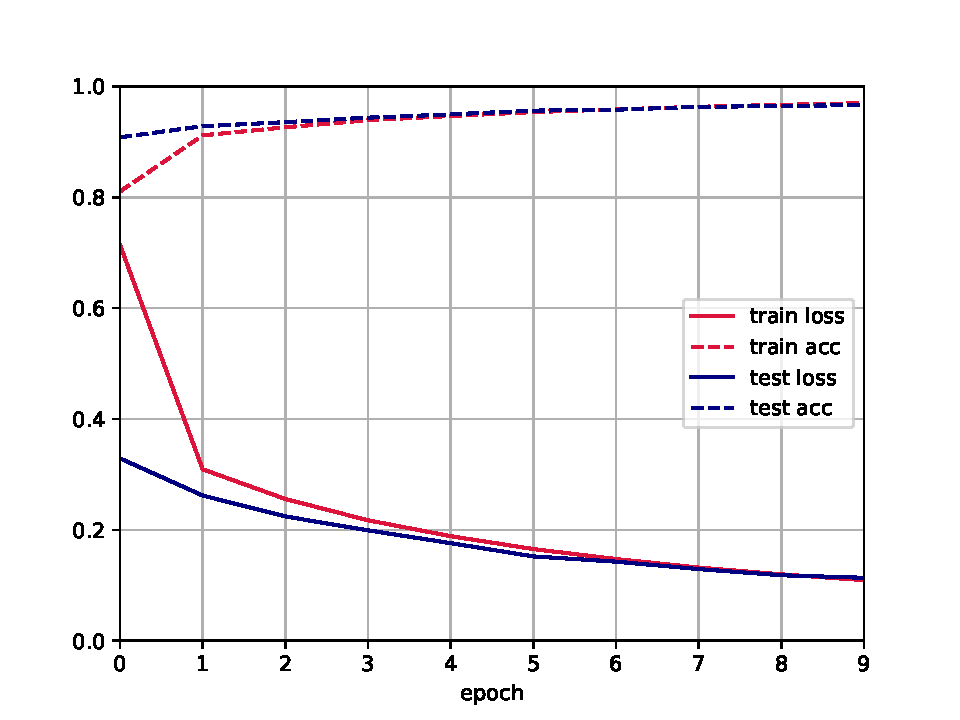
\includegraphics[width=\linewidth]{final_plot}

      Code:

      \begin{lstlisting}[language=Python]
n_inputs = 'not implemented'
n_hiddens = 'not implemented'
n_outputs = 'not implemented'

W1 = 'not implemented'
b1 = 'not implemented'
W2 = 'not implemented'
b2 = 'not implemented'



def relu(x):
    'not implemented'



def softmax(x):
    'not implemented'



def net(X):
  'not implemented'



def cross_entropy(y_hat, y):
  'not implemented'



def sgd(params, lr=0.1):
  'not implemented'



def train(net, params, train_iter, loss_func=cross_entropy, updater=sgd):
  'not implemented'

\end{lstlisting}

    \item[2.]

    \item[3.]

      Test Accuracy (In Distribution):

      Test Accuracy (Out of Distribution):

      Discussion:

    \item[4.]

    \item[5.]

      \begin{enumerate}
        \item
        \item
        \item
      \end{enumerate}


  \end{enumerate}

\end{answer}


%%%%%%%%%%%%%%%%%%%%%%%%%%%%%%%%%%%%%%%%%%%%%
% Name and Calibration
%%%%%%%%%%%%%%%%%%%%%%%%%%%%%%%%%%%%%%%%%%%%%
\newpage
\subsection*{Name}

\subsection*{Collaborators and Resources}
Whom did you work with, and did you use any resources beyond cs181-textbook and your notes?


\end{document}
